
\begin{frame}{Sur le graphe de départ}
	Reprenons notre entreprise $\dots$\vfill
	\begin{center}
		\includegraphics[scale=0.32]{img/exemple.png}
	\end{center}
\end{frame}

\begin{frame}{Sur le graphe de départ}
	$\dots$ et associons lui un graphe.\vfill
	\begin{center}
		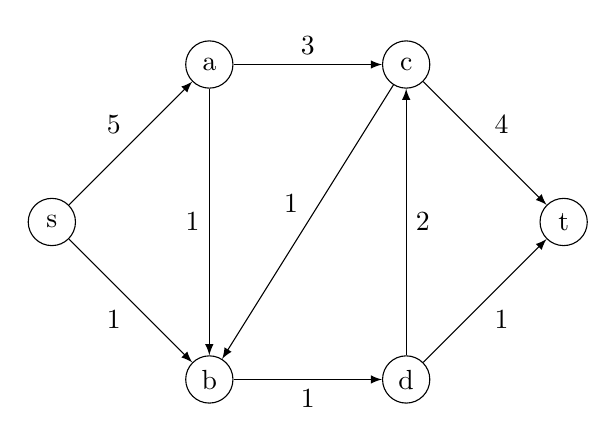
\begin{tikzpicture}
			\tikzset{noeud/.style={circle, draw=black, inner sep=0.1cm, minimum width=0.6cm}, fleche/.style={>=latex, ->}};

				\node[noeud] (s) at (0,0) {s};
				\node[noeud] (a) at (2, 2) {a};
				\node[noeud] (b) at (2, -2) {b};
				\node[noeud] (d) at (4.5, -2) {d};
				\node[noeud] (c) at (4.5, 2) {c};
				\node[noeud] (t) at (6.5,0) {t};

				\draw[fleche] (s) to node[above  left] {$5$} (a);
				\draw[fleche] (s) to node[below  left] {$1$} (b);
				\draw[fleche] (a) to node[       left] {$1$} (b);
				\draw[fleche] (a) to node[above      ] {$3$} (c);
				\draw[fleche] (b) to node[below      ] {$1$} (d);
				\draw[fleche] (c) to node[above  left] {$1$} (b);
				\draw[fleche] (c) to node[above right] {$4$} (t);
				\draw[fleche] (d) to node[      right] {$2$} (c);
				\draw[fleche] (d) to node[below right] {$1$} (t);

		\end{tikzpicture}
	\end{center}
\end{frame}

\begin{frame}{Initialisation}
	\begin{minipage}[c]{0.6\linewidth}
		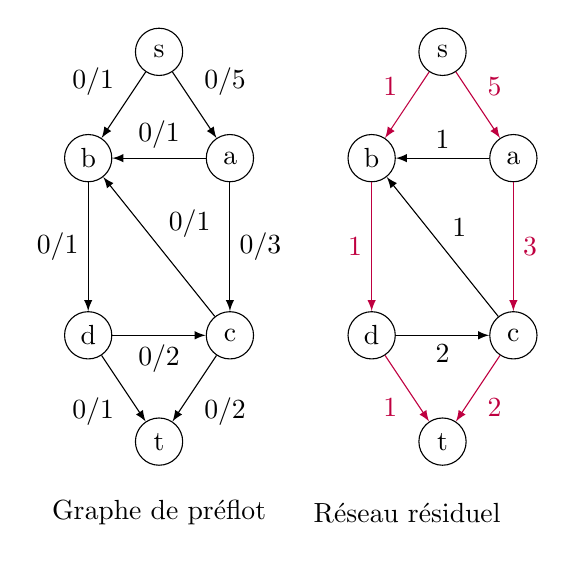
\begin{tikzpicture}[scale=0.45]
			\tikzset{noeud/.style={circle, draw=black, inner sep=0.1cm, minimum width=0.6cm}, fleche/.style={>=latex, ->}};

						\node[noeud] (s1) at (   0,    0) {s};
			\node[noeud] (b1) at (  -2,   -3) {b};
			\node[noeud] (a1) at (   2,   -3) {a};
			\node[noeud] (d1) at (  -2,   -8) {d};
			\node[noeud] (c1) at (   2,   -8) {c};
			\node[noeud] (t1) at (   0,  -11) {t};

			\node[noeud] (s2) at (   8,    0) {s};
			\node[noeud] (b2) at (	 6,   -3) {b};
			\node[noeud] (a2) at (   10,   -3) {a};
			\node[noeud] (d2) at (   6,   -8) {d};
			\node[noeud] (c2) at (   10,   -8) {c};
			\node[noeud] (t2) at (   8,  -11) {t};

			\node at (0,-13) {Graphe de préflot};
			\node at (7,-13) {Réseau résiduel};


			\draw[fleche] (s1) to node[above right] {$0/5$} (a1);
			\draw[fleche] (s1) to node[above  left] {$0/1$} (b1);
			\draw[fleche] (a1) to node[above      ] {$0/1$} (b1);
			\draw[fleche] (a1) to node[      right] {$0/3$} (c1);
			\draw[fleche] (b1) to node[       left] {$0/1$} (d1);
			\draw[fleche] (c1) to node[above right] {$0/1$} (b1);
			\draw[fleche] (c1) to node[below right] {$0/2$} (t1);
			\draw[fleche] (d1) to node[below      ] {$0/2$} (c1);
			\draw[fleche] (d1) to node[below  left] {$0/1$} (t1);

			\draw[fleche, purple] (s2) to node[above right, purple] {$5$} (a2);
			\draw[fleche, purple] (s2) to node[above  left, purple] {$1$} (b2);
			\draw[fleche, purple] (a2) to node[      right, purple] {$3$} (c2);
			\draw[fleche, purple] (b2) to node[       left, purple] {$1$} (d2);
			\draw[fleche, purple] (c2) to node[below right, purple] {$2$} (t2);
			\draw[fleche, purple] (d2) to node[below  left, purple] {$1$} (t2);
			\draw[fleche] (d2) to node[below      ] {$2$} (c2);
			\draw[fleche] (c2) to node[above right] {$1$} (b2);
			\draw[fleche] (a2) to node[above      ] {$1$} (b2);

		\end{tikzpicture}
	\end{minipage}\hfill
	\begin{minipage}[c]{0.3\linewidth}
		\begin{tabular}{|c|c|c|}
			\hline
			$i$ & $e(i)$ & $d(i)$ \\ \hline
			s & $\infty$ & 3* \\ \hline
			a &  0 & 2 \\ \hline
			b &  0 & 2 \\ \hline
			c &  0 & 1 \\ \hline
			d &  0 & 1 \\ \hline
			t &  0 & 0 \\ \hline
		\end{tabular}
	\end{minipage}
\end{frame}

\begin{frame}{Phase 1 - Poussage}
	\begin{minipage}[c]{0.6\linewidth}
		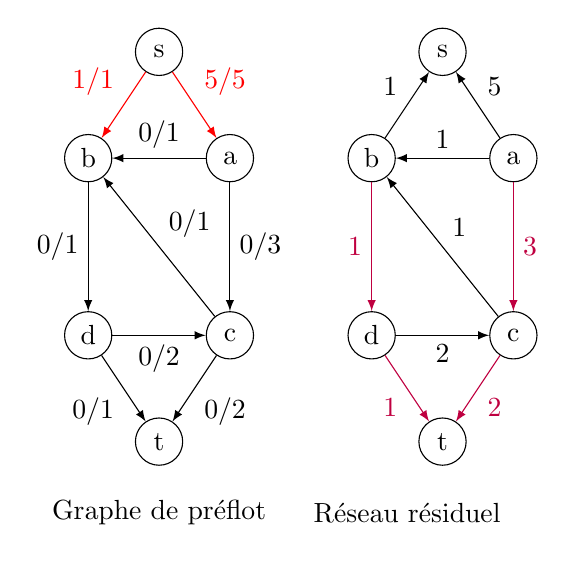
\begin{tikzpicture}[scale=0.45]
			\tikzset{noeud/.style={circle, draw=black, inner sep=0.1cm, minimum width=0.6cm}, fleche/.style={>=latex, ->}};

						\node[noeud] (s1) at (   0,    0) {s};
			\node[noeud] (b1) at (  -2,   -3) {b};
			\node[noeud] (a1) at (   2,   -3) {a};
			\node[noeud] (d1) at (  -2,   -8) {d};
			\node[noeud] (c1) at (   2,   -8) {c};
			\node[noeud] (t1) at (   0,  -11) {t};

			\node[noeud] (s2) at (   8,    0) {s};
			\node[noeud] (b2) at (	 6,   -3) {b};
			\node[noeud] (a2) at (   10,   -3) {a};
			\node[noeud] (d2) at (   6,   -8) {d};
			\node[noeud] (c2) at (   10,   -8) {c};
			\node[noeud] (t2) at (   8,  -11) {t};

			\node at (0,-13) {Graphe de préflot};
			\node at (7,-13) {Réseau résiduel};


			\draw[fleche, red] (s1) to node[above right, red] {$5/5$} (a1);
			\draw[fleche, red] (s1) to node[above  left, red] {$1/1$} (b1);
			\draw[fleche] (a1) to node[above      ] {$0/1$} (b1);
			\draw[fleche] (a1) to node[      right] {$0/3$} (c1);
			\draw[fleche] (b1) to node[       left] {$0/1$} (d1);
			\draw[fleche] (c1) to node[above right] {$0/1$} (b1);
			\draw[fleche] (c1) to node[below right] {$0/2$} (t1);
			\draw[fleche] (d1) to node[below      ] {$0/2$} (c1);
			\draw[fleche] (d1) to node[below  left] {$0/1$} (t1);

			\draw[fleche] (a2) to node[above right] {$5$} (s2);
			\draw[fleche] (b2) to node[above  left] {$1$} (s2);
			\draw[fleche, purple] (a2) to node[      right, purple] {$3$} (c2);
			\draw[fleche, purple] (b2) to node[       left, purple] {$1$} (d2);
			\draw[fleche, purple] (c2) to node[below right, purple] {$2$} (t2);
			\draw[fleche, purple] (d2) to node[below  left, purple] {$1$} (t2);
			\draw[fleche] (d2) to node[below      ] {$2$} (c2);
			\draw[fleche] (c2) to node[above right] {$1$} (b2);
			\draw[fleche] (a2) to node[above      ] {$1$} (b2);

		\end{tikzpicture}
	\end{minipage}\hfill
	\begin{minipage}[c]{0.3\linewidth}
		\begin{tabular}{|c|c|c|}
			\hline
			$i$ & $e(i)$ & $d(i)$ \\ \hline
			\textcolor{blue}{s} & $\infty$ & \textcolor{blue}{6*} \\ \hline
			a &  \textcolor{green}{5} & 2 \\ \hline
			b &  \textcolor{green}{1} & 2 \\ \hline
			c &  0 & 1 \\ \hline
			d &  0 & 1 \\ \hline
			t &  0 & 0 \\ \hline
		\end{tabular}
	\end{minipage}
\end{frame}

\begin{frame}{Phase 1 - Poussage}
	\begin{minipage}[c]{0.6\linewidth}
		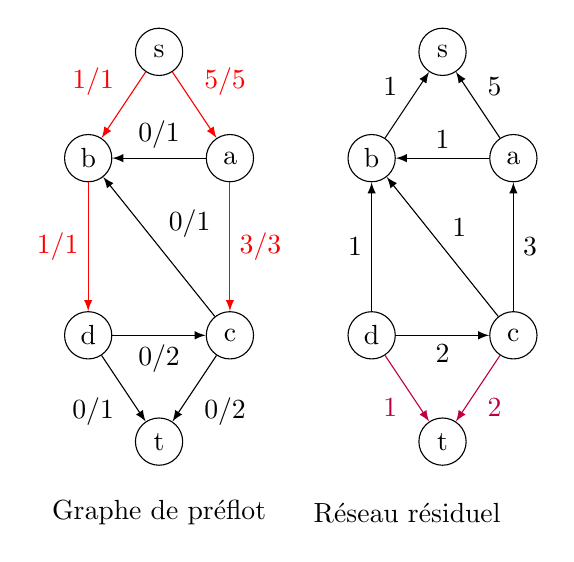
\begin{tikzpicture}[scale=0.45]
			\tikzset{noeud/.style={circle, draw=black, inner sep=0.1cm, minimum width=0.6cm}, fleche/.style={>=latex, ->}};

						\node[noeud] (s1) at (   0,    0) {s};
			\node[noeud] (b1) at (  -2,   -3) {b};
			\node[noeud] (a1) at (   2,   -3) {a};
			\node[noeud] (d1) at (  -2,   -8) {d};
			\node[noeud] (c1) at (   2,   -8) {c};
			\node[noeud] (t1) at (   0,  -11) {t};

			\node[noeud] (s2) at (   8,    0) {s};
			\node[noeud] (b2) at (	 6,   -3) {b};
			\node[noeud] (a2) at (   10,   -3) {a};
			\node[noeud] (d2) at (   6,   -8) {d};
			\node[noeud] (c2) at (   10,   -8) {c};
			\node[noeud] (t2) at (   8,  -11) {t};

			\node at (0,-13) {Graphe de préflot};
			\node at (7,-13) {Réseau résiduel};


			\draw[fleche, red] (s1) to node[above right, red] {$5/5$} (a1);
			\draw[fleche, red] (s1) to node[above  left, red] {$1/1$} (b1);
			\draw[fleche] (a1) to node[above      ] {$0/1$} (b1);
			\draw[fleche, red] (a1) to node[      right, red] {$3/3$} (c1);
			\draw[fleche, red] (b1) to node[       left, red] {$1/1$} (d1);
			\draw[fleche] (c1) to node[above right] {$0/1$} (b1);
			\draw[fleche] (c1) to node[below right] {$0/2$} (t1);
			\draw[fleche] (d1) to node[below      ] {$0/2$} (c1);
			\draw[fleche] (d1) to node[below  left] {$0/1$} (t1);

			\draw[fleche] (a2) to node[above right] {$5$} (s2);
			\draw[fleche] (b2) to node[above  left] {$1$} (s2);
			\draw[fleche] (c2) to node[      right] {$3$} (a2);
			\draw[fleche] (d2) to node[       left] {$1$} (b2);
			\draw[fleche, purple] (c2) to node[below right, purple] {$2$} (t2);
			\draw[fleche, purple] (d2) to node[below  left, purple] {$1$} (t2);
			\draw[fleche] (d2) to node[below      ] {$2$} (c2);
			\draw[fleche] (c2) to node[above right] {$1$} (b2);
			\draw[fleche] (a2) to node[above      ] {$1$} (b2);

		\end{tikzpicture}
	\end{minipage}\hfill
	\begin{minipage}[c]{0.3\linewidth}
		\begin{tabular}{|c|c|c|}
			\hline
			$i$ & $e(i)$ & $d(i)$ \\ \hline
			s & $\infty$ & 6* \\ \hline
			a &  \textcolor{orange}{2} & 2 \\ \hline
			b &  \textcolor{orange}{0} & 2 \\ \hline
			c &  \textcolor{green}{3} & 1 \\ \hline
			d &  \textcolor{green}{1} & 1 \\ \hline
			t &  0 & 0 \\ \hline
		\end{tabular}
	\end{minipage}
\end{frame}

\begin{frame}{Phase 1 - Poussage}
	\begin{minipage}[c]{0.6\linewidth}
		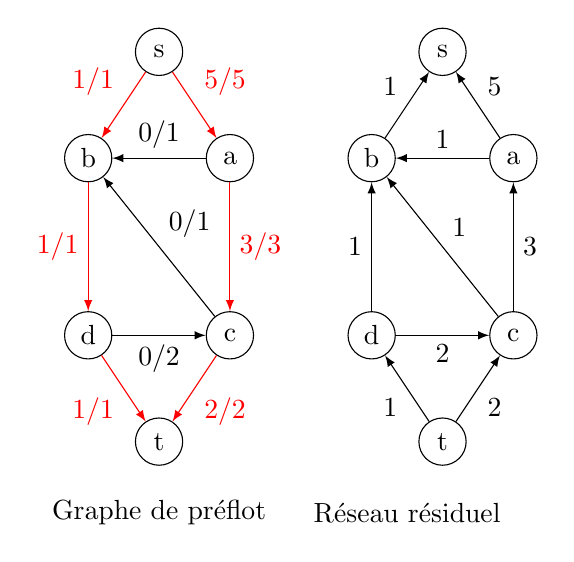
\begin{tikzpicture}[scale=0.45]
			\tikzset{noeud/.style={circle, draw=black, inner sep=0.1cm, minimum width=0.6cm}, fleche/.style={>=latex, ->}};

						\node[noeud] (s1) at (   0,    0) {s};
			\node[noeud] (b1) at (  -2,   -3) {b};
			\node[noeud] (a1) at (   2,   -3) {a};
			\node[noeud] (d1) at (  -2,   -8) {d};
			\node[noeud] (c1) at (   2,   -8) {c};
			\node[noeud] (t1) at (   0,  -11) {t};

			\node[noeud] (s2) at (   8,    0) {s};
			\node[noeud] (b2) at (	 6,   -3) {b};
			\node[noeud] (a2) at (   10,   -3) {a};
			\node[noeud] (d2) at (   6,   -8) {d};
			\node[noeud] (c2) at (   10,   -8) {c};
			\node[noeud] (t2) at (   8,  -11) {t};

			\node at (0,-13) {Graphe de préflot};
			\node at (7,-13) {Réseau résiduel};


			\draw[fleche, red] (s1) to node[above right, red] {$5/5$} (a1);
			\draw[fleche, red] (s1) to node[above  left, red] {$1/1$} (b1);
			\draw[fleche] (a1) to node[above      ] {$0/1$} (b1);
			\draw[fleche, red] (a1) to node[      right, red] {$3/3$} (c1);
			\draw[fleche, red] (b1) to node[       left, red] {$1/1$} (d1);
			\draw[fleche] (c1) to node[above right] {$0/1$} (b1);
			\draw[fleche, red] (c1) to node[below right, red] {$2/2$} (t1);
			\draw[fleche] (d1) to node[below      ] {$0/2$} (c1);
			\draw[fleche, red] (d1) to node[below  left, red] {$1/1$} (t1);

			\draw[fleche] (a2) to node[above right] {$5$} (s2);
			\draw[fleche] (b2) to node[above  left] {$1$} (s2);
			\draw[fleche] (c2) to node[      right] {$3$} (a2);
			\draw[fleche] (d2) to node[       left] {$1$} (b2);
			\draw[fleche] (t2) to node[below right] {$2$} (c2);
			\draw[fleche] (t2) to node[below  left] {$1$} (d2);
			\draw[fleche] (d2) to node[below      ] {$2$} (c2);
			\draw[fleche] (c2) to node[above right] {$1$} (b2);
			\draw[fleche] (a2) to node[above      ] {$1$} (b2);
		\end{tikzpicture}
	\end{minipage}\hfill
	\begin{minipage}[c]{0.3\linewidth}
		\begin{tabular}{|c|c|c|}
			\hline
			$i$ & $e(i)$ & $d(i)$ \\ \hline
			s & $\infty$ & 6* \\ \hline
			a &  \textcolor{orange}{2} & 2 \\ \hline
			b &  0 & 2 \\ \hline
			c &  \textcolor{orange}{1} & 1 \\ \hline
			d &  \textcolor{orange}{0} & 1 \\ \hline
			t &  \textcolor{green}{3} & 0 \\ \hline
		\end{tabular}
	\end{minipage}
\end{frame}

\begin{frame}{Phase 1 - Réétiquetage}
	\begin{minipage}[c]{0.6\linewidth}
		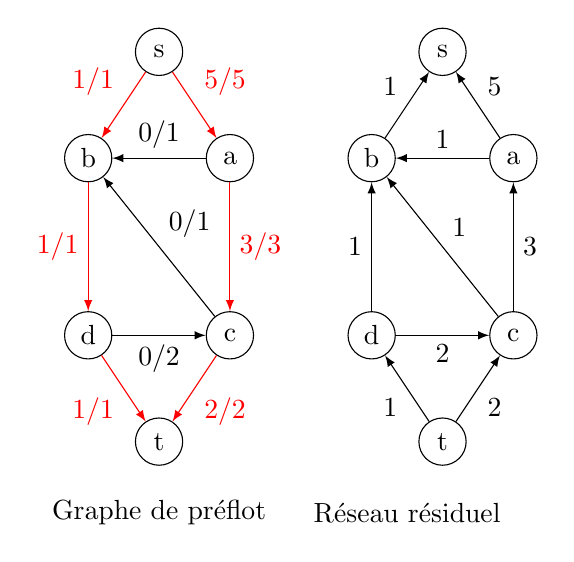
\begin{tikzpicture}[scale=0.45]
			\tikzset{noeud/.style={circle, draw=black, inner sep=0.1cm, minimum width=0.6cm}, fleche/.style={>=latex, ->}};

						\node[noeud] (s1) at (   0,    0) {s};
			\node[noeud] (b1) at (  -2,   -3) {b};
			\node[noeud] (a1) at (   2,   -3) {a};
			\node[noeud] (d1) at (  -2,   -8) {d};
			\node[noeud] (c1) at (   2,   -8) {c};
			\node[noeud] (t1) at (   0,  -11) {t};

			\node[noeud] (s2) at (   8,    0) {s};
			\node[noeud] (b2) at (	 6,   -3) {b};
			\node[noeud] (a2) at (   10,   -3) {a};
			\node[noeud] (d2) at (   6,   -8) {d};
			\node[noeud] (c2) at (   10,   -8) {c};
			\node[noeud] (t2) at (   8,  -11) {t};

			\node at (0,-13) {Graphe de préflot};
			\node at (7,-13) {Réseau résiduel};


			\draw[fleche, red] (s1) to node[above right, red] {$5/5$} (a1);
			\draw[fleche, red] (s1) to node[above  left, red] {$1/1$} (b1);
			\draw[fleche] (a1) to node[above      ] {$0/1$} (b1);
			\draw[fleche, red] (a1) to node[      right, red] {$3/3$} (c1);
			\draw[fleche, red] (b1) to node[       left, red] {$1/1$} (d1);
			\draw[fleche] (c1) to node[above right] {$0/1$} (b1);
			\draw[fleche, red] (c1) to node[below right, red] {$2/2$} (t1);
			\draw[fleche] (d1) to node[below      ] {$0/2$} (c1);
			\draw[fleche, red] (d1) to node[below  left, red] {$1/1$} (t1);

			\draw[fleche] (a2) to node[above right] {$5$} (s2);
			\draw[fleche] (b2) to node[above  left] {$1$} (s2);
			\draw[fleche] (c2) to node[      right] {$3$} (a2);
			\draw[fleche] (d2) to node[       left] {$1$} (b2);
			\draw[fleche] (t2) to node[below right] {$2$} (c2);
			\draw[fleche] (t2) to node[below  left] {$1$} (d2);
			\draw[fleche] (d2) to node[below      ] {$2$} (c2);
			\draw[fleche] (c2) to node[above right] {$1$} (b2);
			\draw[fleche] (a2) to node[above      ] {$1$} (b2);
		\end{tikzpicture}
	\end{minipage}\hfill
	\begin{minipage}[c]{0.3\linewidth}
		\begin{tabular}{|c|c|c|}
			\hline
			$i$ & $e(i)$ & $d(i)$ \\ \hline
			s & $\infty$ & 6* \\ \hline
			a &  \textcolor{orange}{2} & 2 \\ \hline
			b &  0 & 2 \\ \hline
			\textcolor{blue}{c} &  \textcolor{orange}{1} & \textcolor{blue}{3} \\ \hline
			d &  0 & 1 \\ \hline
			t &  \textcolor{green}{3} & 0 \\ \hline
		\end{tabular}
	\end{minipage}
\end{frame}


\begin{frame}{Phase 1 - Réétiquetage}
	\begin{minipage}[c]{0.6\linewidth}
		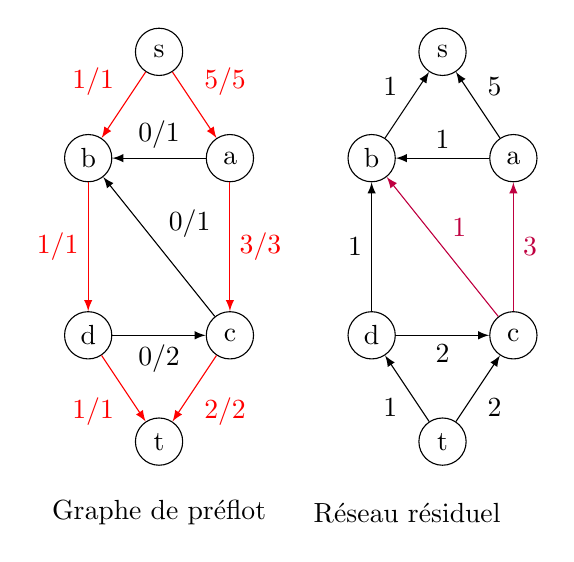
\begin{tikzpicture}[scale=0.45]
			\tikzset{noeud/.style={circle, draw=black, inner sep=0.1cm, minimum width=0.6cm}, fleche/.style={>=latex, ->}};

						\node[noeud] (s1) at (   0,    0) {s};
			\node[noeud] (b1) at (  -2,   -3) {b};
			\node[noeud] (a1) at (   2,   -3) {a};
			\node[noeud] (d1) at (  -2,   -8) {d};
			\node[noeud] (c1) at (   2,   -8) {c};
			\node[noeud] (t1) at (   0,  -11) {t};

			\node[noeud] (s2) at (   8,    0) {s};
			\node[noeud] (b2) at (	 6,   -3) {b};
			\node[noeud] (a2) at (   10,   -3) {a};
			\node[noeud] (d2) at (   6,   -8) {d};
			\node[noeud] (c2) at (   10,   -8) {c};
			\node[noeud] (t2) at (   8,  -11) {t};

			\node at (0,-13) {Graphe de préflot};
			\node at (7,-13) {Réseau résiduel};


			\draw[fleche, red] (s1) to node[above right, red] {$5/5$} (a1);
			\draw[fleche, red] (s1) to node[above  left, red] {$1/1$} (b1);
			\draw[fleche] (a1) to node[above      ] {$0/1$} (b1);
			\draw[fleche, red] (a1) to node[      right, red] {$3/3$} (c1);
			\draw[fleche, red] (b1) to node[       left, red] {$1/1$} (d1);
			\draw[fleche] (c1) to node[above right] {$0/1$} (b1);
			\draw[fleche, red] (c1) to node[below right, red] {$2/2$} (t1);
			\draw[fleche] (d1) to node[below      ] {$0/2$} (c1);
			\draw[fleche, red] (d1) to node[below  left, red] {$1/1$} (t1);

			\draw[fleche] (a2) to node[above right] {$5$} (s2);
			\draw[fleche] (b2) to node[above  left] {$1$} (s2);
			\draw[fleche, purple] (c2) to node[      right, purple] {$3$} (a2);
			\draw[fleche] (d2) to node[       left] {$1$} (b2);
			\draw[fleche] (t2) to node[below right] {$2$} (c2);
			\draw[fleche] (t2) to node[below  left] {$1$} (d2);
			\draw[fleche] (d2) to node[below      ] {$2$} (c2);
			\draw[fleche, purple] (c2) to node[above right, purple] {$1$} (b2);
			\draw[fleche] (a2) to node[above      ] {$1$} (b2);
		\end{tikzpicture}
	\end{minipage}\hfill
	\begin{minipage}[c]{0.3\linewidth}
		\begin{tabular}{|c|c|c|}
			\hline
			$i$ & $e(i)$ & $d(i)$ \\ \hline
			s & $\infty$ & 6* \\ \hline
			a &  \textcolor{orange}{2} & 2 \\ \hline
			b &  0 & 2 \\ \hline
			\textcolor{blue}{c} &  \textcolor{orange}{1} & \textcolor{blue}{3} \\ \hline
			d &  0 & 1 \\ \hline
			t &  \textcolor{green}{3} & 0 \\ \hline
		\end{tabular}
	\end{minipage}
\end{frame}

\begin{frame}{Phase 2 - Poussage}
	\begin{minipage}[c]{0.6\linewidth}
		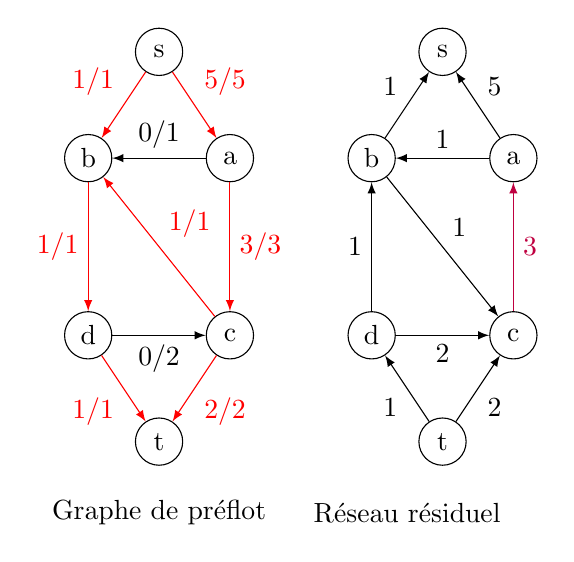
\begin{tikzpicture}[scale=0.45]
			\tikzset{noeud/.style={circle, draw=black, inner sep=0.1cm, minimum width=0.6cm}, fleche/.style={>=latex, ->}};

						\node[noeud] (s1) at (   0,    0) {s};
			\node[noeud] (b1) at (  -2,   -3) {b};
			\node[noeud] (a1) at (   2,   -3) {a};
			\node[noeud] (d1) at (  -2,   -8) {d};
			\node[noeud] (c1) at (   2,   -8) {c};
			\node[noeud] (t1) at (   0,  -11) {t};

			\node[noeud] (s2) at (   8,    0) {s};
			\node[noeud] (b2) at (	 6,   -3) {b};
			\node[noeud] (a2) at (   10,   -3) {a};
			\node[noeud] (d2) at (   6,   -8) {d};
			\node[noeud] (c2) at (   10,   -8) {c};
			\node[noeud] (t2) at (   8,  -11) {t};

			\node at (0,-13) {Graphe de préflot};
			\node at (7,-13) {Réseau résiduel};


			\draw[fleche, red] (s1) to node[above right, red] {$5/5$} (a1);
			\draw[fleche, red] (s1) to node[above  left, red] {$1/1$} (b1);
			\draw[fleche] (a1) to node[above      ] {$0/1$} (b1);
			\draw[fleche, red] (a1) to node[      right, red] {$3/3$} (c1);
			\draw[fleche, red] (b1) to node[       left, red] {$1/1$} (d1);
			\draw[fleche, red] (c1) to node[above right] {$1/1$} (b1);
			\draw[fleche, red] (c1) to node[below right, red] {$2/2$} (t1);
			\draw[fleche] (d1) to node[below      ] {$0/2$} (c1);
			\draw[fleche, red] (d1) to node[below  left, red] {$1/1$} (t1);

			\draw[fleche] (a2) to node[above right] {$5$} (s2);
			\draw[fleche] (b2) to node[above  left] {$1$} (s2);
			\draw[fleche, purple] (c2) to node[      right, purple] {$3$} (a2);
			\draw[fleche] (d2) to node[       left] {$1$} (b2);
			\draw[fleche] (t2) to node[below right] {$2$} (c2);
			\draw[fleche] (t2) to node[below  left] {$1$} (d2);
			\draw[fleche] (d2) to node[below      ] {$2$} (c2);
			\draw[fleche] (b2) to node[above right] {$1$} (c2);
			\draw[fleche] (a2) to node[above      ] {$1$} (b2);
		\end{tikzpicture}
	\end{minipage}\hfill
	\begin{minipage}[c]{0.3\linewidth}
		\begin{tabular}{|c|c|c|}
			\hline
			$i$ & $e(i)$ & $d(i)$ \\ \hline
			s & $\infty$ & 6* \\ \hline
			a &  \textcolor{orange}{2} & 2 \\ \hline
			b &  \textcolor{green}{1} & 2 \\ \hline
			c &  0 & 3 \\ \hline
			d &  0 & 1 \\ \hline
			t &  \textcolor{green}{3} & 0 \\ \hline
		\end{tabular}
	\end{minipage}
\end{frame}

\begin{frame}{Phase 2 - Réétiquetage}
	\begin{minipage}[c]{0.6\linewidth}
		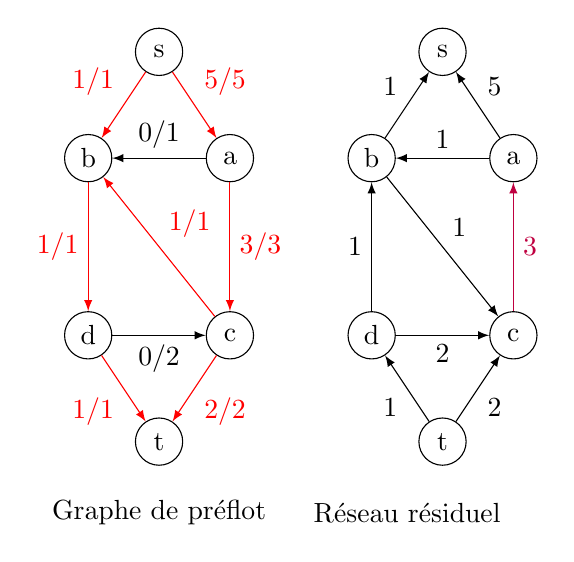
\begin{tikzpicture}[scale=0.45]
			\tikzset{noeud/.style={circle, draw=black, inner sep=0.1cm, minimum width=0.6cm}, fleche/.style={>=latex, ->}};

						\node[noeud] (s1) at (   0,    0) {s};
			\node[noeud] (b1) at (  -2,   -3) {b};
			\node[noeud] (a1) at (   2,   -3) {a};
			\node[noeud] (d1) at (  -2,   -8) {d};
			\node[noeud] (c1) at (   2,   -8) {c};
			\node[noeud] (t1) at (   0,  -11) {t};

			\node[noeud] (s2) at (   8,    0) {s};
			\node[noeud] (b2) at (	 6,   -3) {b};
			\node[noeud] (a2) at (   10,   -3) {a};
			\node[noeud] (d2) at (   6,   -8) {d};
			\node[noeud] (c2) at (   10,   -8) {c};
			\node[noeud] (t2) at (   8,  -11) {t};

			\node at (0,-13) {Graphe de préflot};
			\node at (7,-13) {Réseau résiduel};


			\draw[fleche, red] (s1) to node[above right, red] {$5/5$} (a1);
			\draw[fleche, red] (s1) to node[above  left, red] {$1/1$} (b1);
			\draw[fleche] (a1) to node[above      ] {$0/1$} (b1);
			\draw[fleche, red] (a1) to node[      right, red] {$3/3$} (c1);
			\draw[fleche, red] (b1) to node[       left, red] {$1/1$} (d1);
			\draw[fleche, red] (c1) to node[above right] {$1/1$} (b1);
			\draw[fleche, red] (c1) to node[below right, red] {$2/2$} (t1);
			\draw[fleche] (d1) to node[below      ] {$0/2$} (c1);
			\draw[fleche, red] (d1) to node[below  left, red] {$1/1$} (t1);

			\draw[fleche] (a2) to node[above right] {$5$} (s2);
			\draw[fleche] (b2) to node[above  left] {$1$} (s2);
			\draw[fleche, purple] (c2) to node[      right, purple] {$3$} (a2);
			\draw[fleche] (d2) to node[       left] {$1$} (b2);
			\draw[fleche] (t2) to node[below right] {$2$} (c2);
			\draw[fleche] (t2) to node[below  left] {$1$} (d2);
			\draw[fleche] (d2) to node[below      ] {$2$} (c2);
			\draw[fleche] (b2) to node[above right] {$1$} (c2);
			\draw[fleche] (a2) to node[above      ] {$1$} (b2);

		\end{tikzpicture}
	\end{minipage}\hfill
	\begin{minipage}[c]{0.3\linewidth}
		\begin{tabular}{|c|c|c|}
			\hline
			$i$ & $e(i)$ & $d(i)$ \\ \hline
			s & $\infty$ & 6* \\ \hline
			a &  \textcolor{orange}{2} & 2 \\ \hline
			\textcolor{blue}{b} &  \textcolor{orange}{1} & \textcolor{blue}{4} \\ \hline
			c &  0 & 3 \\ \hline
			d &  0 & 1 \\ \hline
			t &  \textcolor{green}{3} & 0 \\ \hline
		\end{tabular}
	\end{minipage}
\end{frame}


\begin{frame}{Phase 2 - Réétiquetage}
	\begin{minipage}[c]{0.6\linewidth}
		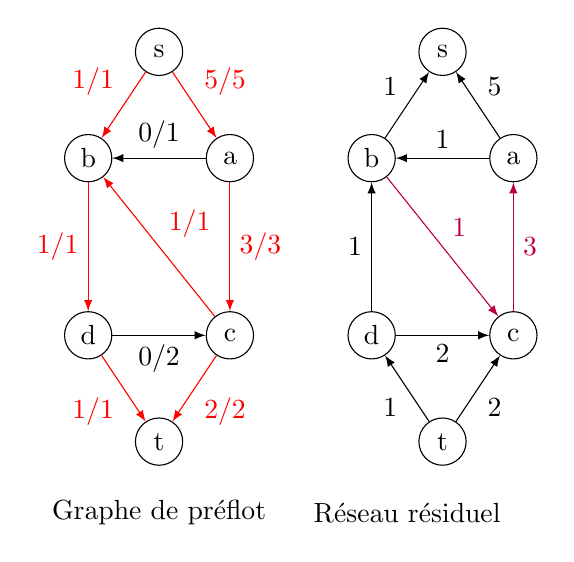
\begin{tikzpicture}[scale=0.45]
			\tikzset{noeud/.style={circle, draw=black, inner sep=0.1cm, minimum width=0.6cm}, fleche/.style={>=latex, ->}};

						\node[noeud] (s1) at (   0,    0) {s};
			\node[noeud] (b1) at (  -2,   -3) {b};
			\node[noeud] (a1) at (   2,   -3) {a};
			\node[noeud] (d1) at (  -2,   -8) {d};
			\node[noeud] (c1) at (   2,   -8) {c};
			\node[noeud] (t1) at (   0,  -11) {t};

			\node[noeud] (s2) at (   8,    0) {s};
			\node[noeud] (b2) at (	 6,   -3) {b};
			\node[noeud] (a2) at (   10,   -3) {a};
			\node[noeud] (d2) at (   6,   -8) {d};
			\node[noeud] (c2) at (   10,   -8) {c};
			\node[noeud] (t2) at (   8,  -11) {t};

			\node at (0,-13) {Graphe de préflot};
			\node at (7,-13) {Réseau résiduel};


			\draw[fleche, red] (s1) to node[above right, red] {$5/5$} (a1);
			\draw[fleche, red] (s1) to node[above  left, red] {$1/1$} (b1);
			\draw[fleche] (a1) to node[above      ] {$0/1$} (b1);
			\draw[fleche, red] (a1) to node[      right, red] {$3/3$} (c1);
			\draw[fleche, red] (b1) to node[       left, red] {$1/1$} (d1);
			\draw[fleche, red] (c1) to node[above right] {$1/1$} (b1);
			\draw[fleche, red] (c1) to node[below right, red] {$2/2$} (t1);
			\draw[fleche] (d1) to node[below      ] {$0/2$} (c1);
			\draw[fleche, red] (d1) to node[below  left, red] {$1/1$} (t1);

			\draw[fleche] (a2) to node[above right] {$5$} (s2);
			\draw[fleche] (b2) to node[above  left] {$1$} (s2);
			\draw[fleche, purple] (c2) to node[      right, purple] {$3$} (a2);
			\draw[fleche] (d2) to node[       left] {$1$} (b2);
			\draw[fleche] (t2) to node[below right] {$2$} (c2);
			\draw[fleche] (t2) to node[below  left] {$1$} (d2);
			\draw[fleche] (d2) to node[below      ] {$2$} (c2);
			\draw[fleche, purple] (b2) to node[above right, purple] {$1$} (c2);
			\draw[fleche] (a2) to node[above      ] {$1$} (b2);

		\end{tikzpicture}
	\end{minipage}\hfill
	\begin{minipage}[c]{0.3\linewidth}
		\begin{tabular}{|c|c|c|}
			\hline
			$i$ & $e(i)$ & $d(i)$ \\ \hline
			s & $\infty$ & 6* \\ \hline
			a &  \textcolor{orange}{2} & 2 \\ \hline
			\textcolor{blue}{b} &  \textcolor{orange}{1} & \textcolor{blue}{4} \\ \hline
			c &  0 & 3 \\ \hline
			d &  0 & 1 \\ \hline
			t &  \textcolor{green}{3} & 0 \\ \hline
		\end{tabular}
	\end{minipage}
\end{frame}

\begin{frame}{Phase 3 - Poussage}
	\begin{minipage}[c]{0.6\linewidth}
		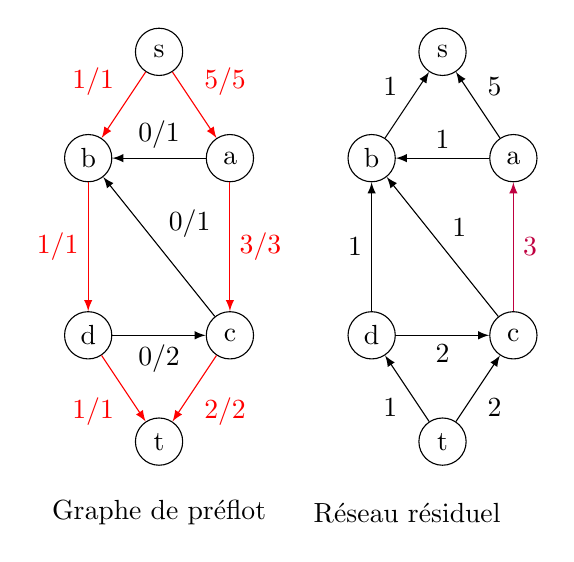
\begin{tikzpicture}[scale=0.45]
			\tikzset{noeud/.style={circle, draw=black, inner sep=0.1cm, minimum width=0.6cm}, fleche/.style={>=latex, ->}};

						\node[noeud] (s1) at (   0,    0) {s};
			\node[noeud] (b1) at (  -2,   -3) {b};
			\node[noeud] (a1) at (   2,   -3) {a};
			\node[noeud] (d1) at (  -2,   -8) {d};
			\node[noeud] (c1) at (   2,   -8) {c};
			\node[noeud] (t1) at (   0,  -11) {t};

			\node[noeud] (s2) at (   8,    0) {s};
			\node[noeud] (b2) at (	 6,   -3) {b};
			\node[noeud] (a2) at (   10,   -3) {a};
			\node[noeud] (d2) at (   6,   -8) {d};
			\node[noeud] (c2) at (   10,   -8) {c};
			\node[noeud] (t2) at (   8,  -11) {t};

			\node at (0,-13) {Graphe de préflot};
			\node at (7,-13) {Réseau résiduel};


			\draw[fleche, red] (s1) to node[above right, red] {$5/5$} (a1);
			\draw[fleche, red] (s1) to node[above  left, red] {$1/1$} (b1);
			\draw[fleche] (a1) to node[above      ] {$0/1$} (b1);
			\draw[fleche, red] (a1) to node[      right, red] {$3/3$} (c1);
			\draw[fleche, red] (b1) to node[       left, red] {$1/1$} (d1);
			\draw[fleche] (c1) to node[above right] {$0/1$} (b1);
			\draw[fleche, red] (c1) to node[below right, red] {$2/2$} (t1);
			\draw[fleche] (d1) to node[below      ] {$0/2$} (c1);
			\draw[fleche, red] (d1) to node[below  left, red] {$1/1$} (t1);

			\draw[fleche] (a2) to node[above right] {$5$} (s2);
			\draw[fleche] (b2) to node[above  left] {$1$} (s2);
			\draw[fleche, purple] (c2) to node[      right, purple] {$3$} (a2);
			\draw[fleche] (d2) to node[       left] {$1$} (b2);
			\draw[fleche] (t2) to node[below right] {$2$} (c2);
			\draw[fleche] (t2) to node[below  left] {$1$} (d2);
			\draw[fleche] (d2) to node[below      ] {$2$} (c2);
			\draw[fleche] (c2) to node[above right] {$1$} (b2);
			\draw[fleche] (a2) to node[above      ] {$1$} (b2);

		\end{tikzpicture}
	\end{minipage}\hfill
	\begin{minipage}[c]{0.3\linewidth}
		\begin{tabular}{|c|c|c|}
			\hline
			$i$ & $e(i)$ & $d(i)$ \\ \hline
			s & $\infty$ & 6* \\ \hline
			a &  \textcolor{orange}{2} & 2 \\ \hline
			b &  0 & 4 \\ \hline
			c &  \textcolor{green}{1} & 3 \\ \hline
			d &  0 & 1 \\ \hline
			t &  \textcolor{green}{3} & 0 \\ \hline
		\end{tabular}
	\end{minipage}
\end{frame}

\begin{frame}{Phase 3 - Poussage}
	\begin{minipage}[c]{0.6\linewidth}
		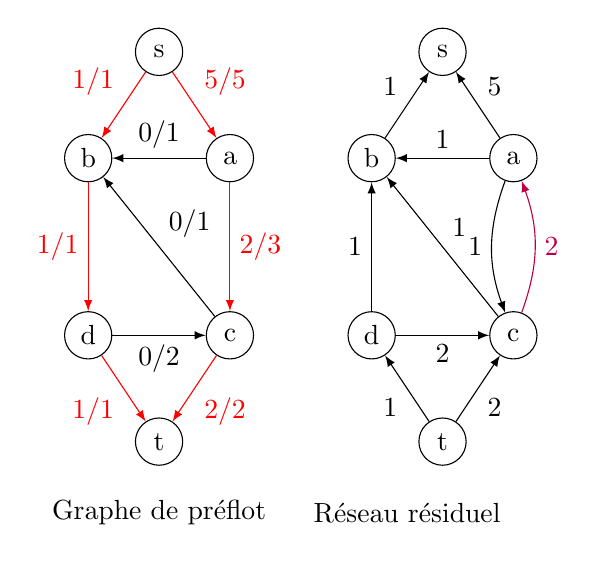
\begin{tikzpicture}[scale=0.45]
			\tikzset{noeud/.style={circle, draw=black, inner sep=0.1cm, minimum width=0.6cm}, fleche/.style={>=latex, ->}};

						\node[noeud] (s1) at (   0,    0) {s};
			\node[noeud] (b1) at (  -2,   -3) {b};
			\node[noeud] (a1) at (   2,   -3) {a};
			\node[noeud] (d1) at (  -2,   -8) {d};
			\node[noeud] (c1) at (   2,   -8) {c};
			\node[noeud] (t1) at (   0,  -11) {t};

			\node[noeud] (s2) at (   8,    0) {s};
			\node[noeud] (b2) at (	 6,   -3) {b};
			\node[noeud] (a2) at (   10,   -3) {a};
			\node[noeud] (d2) at (   6,   -8) {d};
			\node[noeud] (c2) at (   10,   -8) {c};
			\node[noeud] (t2) at (   8,  -11) {t};

			\node at (0,-13) {Graphe de préflot};
			\node at (7,-13) {Réseau résiduel};


			\draw[fleche, red] (s1) to node[above right, red] {$5/5$} (a1);
			\draw[fleche, red] (s1) to node[above  left, red] {$1/1$} (b1);
			\draw[fleche] (a1) to node[above      ] {$0/1$} (b1);
			\draw[fleche, red] (a1) to node[      right, red] {$2/3$} (c1);
			\draw[fleche, red] (b1) to node[       left, red] {$1/1$} (d1);
			\draw[fleche] (c1) to node[above right] {$0/1$} (b1);
			\draw[fleche, red] (c1) to node[below right, red] {$2/2$} (t1);
			\draw[fleche] (d1) to node[below      ] {$0/2$} (c1);
			\draw[fleche, red] (d1) to node[below  left, red] {$1/1$} (t1);

			\draw[fleche] (a2) to node[above right] {$5$} (s2);
			\draw[fleche] (b2) to node[above  left] {$1$} (s2);
			\draw[fleche, purple] (c2) to[out= 70, in=290] node[      right, purple] {$2$} (a2);
			\draw[fleche] (a2) to[out=250, in=110] node[       left] {$1$} (c2);
			\draw[fleche] (d2) to node[       left] {$1$} (b2);
			\draw[fleche] (t2) to node[below right] {$2$} (c2);
			\draw[fleche] (t2) to node[below  left] {$1$} (d2);
			\draw[fleche] (d2) to node[below      ] {$2$} (c2);
			\draw[fleche] (c2) to node[above right] {$1$} (b2);
			\draw[fleche] (a2) to node[above      ] {$1$} (b2);

		\end{tikzpicture}
	\end{minipage}\hfill
	\begin{minipage}[c]{0.3\linewidth}
		\begin{tabular}{|c|c|c|}
			\hline
			$i$ & $e(i)$ & $d(i)$ \\ \hline
			s & $\infty$ & 6* \\ \hline
			a &  \textcolor{green}{3} & 2 \\ \hline
			b &  0 & 4 \\ \hline
			c &  0 & 3 \\ \hline
			d &  0 & 1 \\ \hline
			t &  \textcolor{green}{3} & 0 \\ \hline
		\end{tabular}
	\end{minipage}
\end{frame}


\begin{frame}{Phase 3 - Réétiquetage}
	\begin{minipage}[c]{0.6\linewidth}
		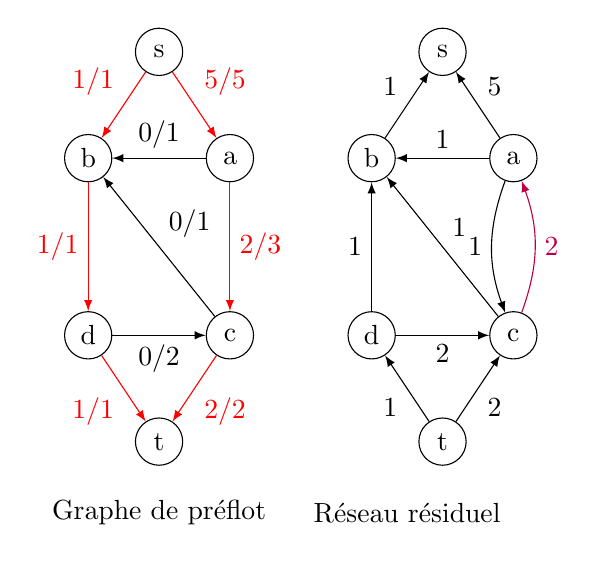
\begin{tikzpicture}[scale=0.45]
			\tikzset{noeud/.style={circle, draw=black, inner sep=0.1cm, minimum width=0.6cm}, fleche/.style={>=latex, ->}};

						\node[noeud] (s1) at (   0,    0) {s};
			\node[noeud] (b1) at (  -2,   -3) {b};
			\node[noeud] (a1) at (   2,   -3) {a};
			\node[noeud] (d1) at (  -2,   -8) {d};
			\node[noeud] (c1) at (   2,   -8) {c};
			\node[noeud] (t1) at (   0,  -11) {t};

			\node[noeud] (s2) at (   8,    0) {s};
			\node[noeud] (b2) at (	 6,   -3) {b};
			\node[noeud] (a2) at (   10,   -3) {a};
			\node[noeud] (d2) at (   6,   -8) {d};
			\node[noeud] (c2) at (   10,   -8) {c};
			\node[noeud] (t2) at (   8,  -11) {t};

			\node at (0,-13) {Graphe de préflot};
			\node at (7,-13) {Réseau résiduel};


			\draw[fleche, red] (s1) to node[above right, red] {$5/5$} (a1);
			\draw[fleche, red] (s1) to node[above  left, red] {$1/1$} (b1);
			\draw[fleche] (a1) to node[above      ] {$0/1$} (b1);
			\draw[fleche, red] (a1) to node[      right, red] {$2/3$} (c1);
			\draw[fleche, red] (b1) to node[       left, red] {$1/1$} (d1);
			\draw[fleche] (c1) to node[above right] {$0/1$} (b1);
			\draw[fleche, red] (c1) to node[below right, red] {$2/2$} (t1);
			\draw[fleche] (d1) to node[below      ] {$0/2$} (c1);
			\draw[fleche, red] (d1) to node[below  left, red] {$1/1$} (t1);

			\draw[fleche] (a2) to node[above right] {$5$} (s2);
			\draw[fleche] (b2) to node[above  left] {$1$} (s2);
			\draw[fleche, purple] (c2) to[out= 70, in=290] node[      right, purple] {$2$} (a2);
			\draw[fleche] (a2) to[out=250, in=110] node[       left] {$1$} (c2);
			\draw[fleche] (d2) to node[       left] {$1$} (b2);
			\draw[fleche] (t2) to node[below right] {$2$} (c2);
			\draw[fleche] (t2) to node[below  left] {$1$} (d2);
			\draw[fleche] (d2) to node[below      ] {$2$} (c2);
			\draw[fleche] (c2) to node[above right] {$1$} (b2);
			\draw[fleche] (a2) to node[above      ] {$1$} (b2);

		\end{tikzpicture}
	\end{minipage}\hfill
	\begin{minipage}[c]{0.3\linewidth}
		\begin{tabular}{|c|c|c|}
			\hline
			$i$ & $e(i)$ & $d(i)$ \\ \hline
			s & $\infty$ & 6* \\ \hline
			\textcolor{blue}{a} &  \textcolor{orange}{3} & \textcolor{blue}{4} \\ \hline
			b &  0 & 4 \\ \hline
			c &  0 & 3 \\ \hline
			d &  0 & 1 \\ \hline
			t &  \textcolor{green}{3} & 0 \\ \hline
		\end{tabular}
	\end{minipage}
\end{frame}

\begin{frame}{Phase 3 - Réétiquetage}
	\begin{minipage}[c]{0.6\linewidth}
		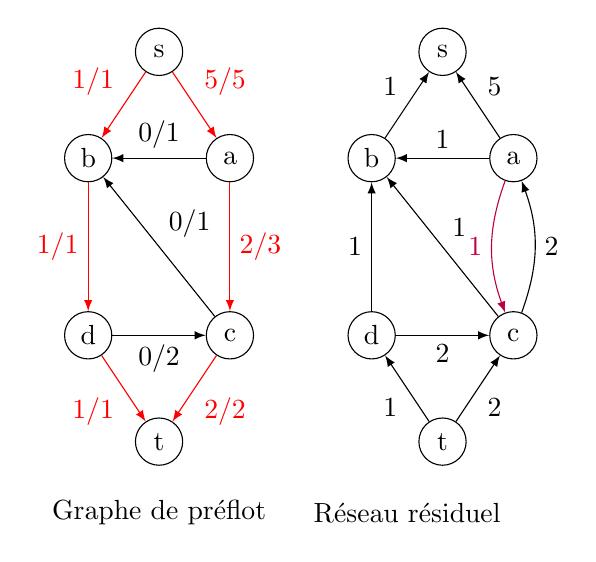
\begin{tikzpicture}[scale=0.45]
			\tikzset{noeud/.style={circle, draw=black, inner sep=0.1cm, minimum width=0.6cm}, fleche/.style={>=latex, ->}};

						\node[noeud] (s1) at (   0,    0) {s};
			\node[noeud] (b1) at (  -2,   -3) {b};
			\node[noeud] (a1) at (   2,   -3) {a};
			\node[noeud] (d1) at (  -2,   -8) {d};
			\node[noeud] (c1) at (   2,   -8) {c};
			\node[noeud] (t1) at (   0,  -11) {t};

			\node[noeud] (s2) at (   8,    0) {s};
			\node[noeud] (b2) at (	 6,   -3) {b};
			\node[noeud] (a2) at (   10,   -3) {a};
			\node[noeud] (d2) at (   6,   -8) {d};
			\node[noeud] (c2) at (   10,   -8) {c};
			\node[noeud] (t2) at (   8,  -11) {t};

			\node at (0,-13) {Graphe de préflot};
			\node at (7,-13) {Réseau résiduel};


			\draw[fleche, red] (s1) to node[above right, red] {$5/5$} (a1);
			\draw[fleche, red] (s1) to node[above  left, red] {$1/1$} (b1);
			\draw[fleche] (a1) to node[above      ] {$0/1$} (b1);
			\draw[fleche, red] (a1) to node[      right, red] {$2/3$} (c1);
			\draw[fleche, red] (b1) to node[       left, red] {$1/1$} (d1);
			\draw[fleche] (c1) to node[above right] {$0/1$} (b1);
			\draw[fleche, red] (c1) to node[below right, red] {$2/2$} (t1);
			\draw[fleche] (d1) to node[below      ] {$0/2$} (c1);
			\draw[fleche, red] (d1) to node[below  left, red] {$1/1$} (t1);

			\draw[fleche] (a2) to node[above right] {$5$} (s2);
			\draw[fleche] (b2) to node[above  left] {$1$} (s2);
			\draw[fleche] (c2) to[out= 70, in=290] node[      right] {$2$} (a2);
			\draw[fleche, purple] (a2) to[out=250, in=110] node[       left, purple] {$1$} (c2);
			\draw[fleche] (d2) to node[       left] {$1$} (b2);
			\draw[fleche] (t2) to node[below right] {$2$} (c2);
			\draw[fleche] (t2) to node[below  left] {$1$} (d2);
			\draw[fleche] (d2) to node[below      ] {$2$} (c2);
			\draw[fleche] (c2) to node[above right] {$1$} (b2);
			\draw[fleche] (a2) to node[above      ] {$1$} (b2);

		\end{tikzpicture}
	\end{minipage}\hfill
	\begin{minipage}[c]{0.3\linewidth}
		\begin{tabular}{|c|c|c|}
			\hline
			$i$ & $e(i)$ & $d(i)$ \\ \hline
			s & $\infty$ & 6* \\ \hline
			\textcolor{blue}{a} &  \textcolor{orange}{3} & \textcolor{blue}{4} \\ \hline
			b &  0 & 4 \\ \hline
			c &  0 & 3 \\ \hline
			d &  0 & 1 \\ \hline
			t &  \textcolor{green}{3} & 0 \\ \hline
		\end{tabular}
	\end{minipage}
\end{frame}



\begin{frame}{Quelques tours d'algorithme plus tard...}
	\begin{minipage}[c]{0.6\linewidth}
		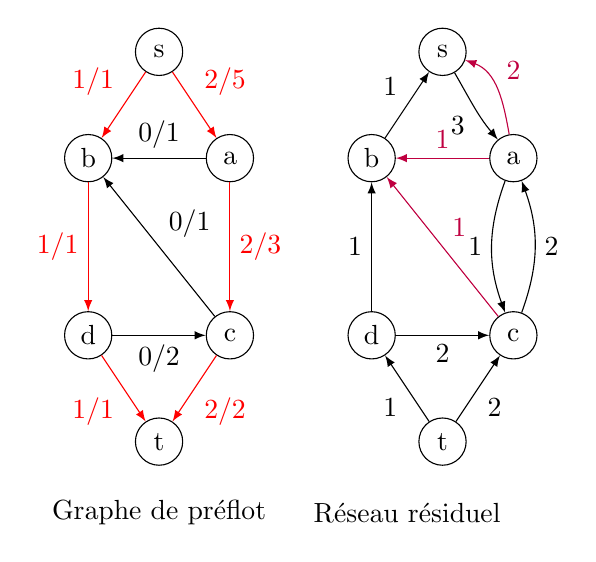
\begin{tikzpicture}[scale=0.45]
			\tikzset{noeud/.style={circle, draw=black, inner sep=0.1cm, minimum width=0.6cm}, fleche/.style={>=latex, ->}};

						\node[noeud] (s1) at (   0,    0) {s};
			\node[noeud] (b1) at (  -2,   -3) {b};
			\node[noeud] (a1) at (   2,   -3) {a};
			\node[noeud] (d1) at (  -2,   -8) {d};
			\node[noeud] (c1) at (   2,   -8) {c};
			\node[noeud] (t1) at (   0,  -11) {t};

			\node[noeud] (s2) at (   8,    0) {s};
			\node[noeud] (b2) at (	 6,   -3) {b};
			\node[noeud] (a2) at (   10,   -3) {a};
			\node[noeud] (d2) at (   6,   -8) {d};
			\node[noeud] (c2) at (   10,   -8) {c};
			\node[noeud] (t2) at (   8,  -11) {t};

			\node at (0,-13) {Graphe de préflot};
			\node at (7,-13) {Réseau résiduel};


			\draw[fleche, red] (s1) to node[above right, red] {$2/5$} (a1);
			\draw[fleche, red] (s1) to node[above  left, red] {$1/1$} (b1);
			\draw[fleche] (a1) to node[above      ] {$0/1$} (b1);
			\draw[fleche, red] (a1) to node[      right, red] {$2/3$} (c1);
			\draw[fleche, red] (b1) to node[       left, red] {$1/1$} (d1);
			\draw[fleche] (c1) to node[above right] {$0/1$} (b1);
			\draw[fleche, red] (c1) to node[below right, red] {$2/2$} (t1);
			\draw[fleche] (d1) to node[below      ] {$0/2$} (c1);
			\draw[fleche, red] (d1) to node[below  left, red] {$1/1$} (t1);

			\draw[fleche, purple] (a2) to[out=100, in=340] node[above right, purple] {$2$} (s2);
			\draw[fleche] (s2) to[out=300, in=130] node[below left] {$3$} (a2);
			\draw[fleche] (b2) to node[above  left] {$1$} (s2);
			\draw[fleche] (c2) to[out= 70, in=290] node[      right] {$2$} (a2);
			\draw[fleche] (a2) to[out=250, in=110] node[       left] {$1$} (c2);
			\draw[fleche] (d2) to node[       left] {$1$} (b2);
			\draw[fleche] (t2) to node[below right] {$2$} (c2);
			\draw[fleche] (t2) to node[below  left] {$1$} (d2);
			\draw[fleche] (d2) to node[below      ] {$2$} (c2);
			\draw[fleche, purple] (c2) to node[above right, purple] {$1$} (b2);
			\draw[fleche, purple] (a2) to node[above      , purple] {$1$} (b2);

		\end{tikzpicture}
	\end{minipage}\hfill
	\begin{minipage}[c]{0.3\linewidth}
		\begin{tabular}{|c|c|c|}
			\hline
			$i$ & $e(i)$ & $d(i)$ \\ \hline
			s & $\infty$ & 6* \\ \hline
			a &  0 & 7 \\ \hline
			b &  0 & 6 \\ \hline
			c &  0 & 7 \\ \hline
			d &  0 & 1 \\ \hline
			t &  \textcolor{green}{3} & 0 \\ \hline
		\end{tabular}
	\end{minipage}
\end{frame}



